\section{Motivation to add a third normal component}
\label{sec:motivation-to-add-a-third-normal-component}

As is said in \cref{ch:introduction},
we try to describe more possible shapes by adding a third normal component.
To illustrate that, we plot some of the shapes which are now possible with three normals
but were not possible with only two.
To be able to draw those plots, we are just using two variables, $w$, the upward wind,
and $\theta_l$, the liquid water potential temperature.
To show how the binormal model handles strong winds,
let us consider a scenario with a strong updraft at $w_1$, as well as a strong downdraft at $w_2$.
The way the current binormal model would handle this could look like \cref{fig:plot1}.
\begin{figure}[!htb]
    \centering
    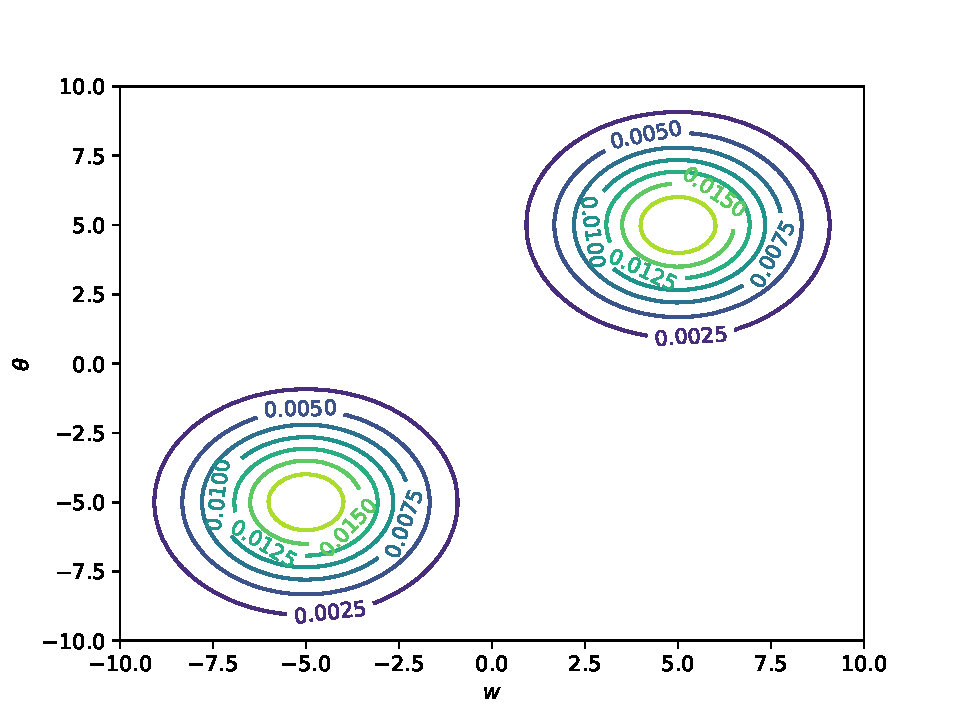
\includegraphics[width=.48\textwidth]{include/figures/plot1}
    \caption{Binormal plot for two strong up-/downdrafts}
    \label{fig:plot1}
    $w_1 = 5$, $w_2 = -5$, $\theta_{l1} = 5$, $\theta_{l2} = -5$,
    $\alpha = 0.5$, $\sigma_w = 2$, $\sigma_{\theta_{l1}} = 2$, $\sigma_{\theta_{l1}} = 2$.
\end{figure}
However, this binormal distribution (\cref{fig:plot1}) does not accurately reflect reality.
In nature, we would not expect such strong bi-modality between the strong up-
and downdrafts at $w_1$ and $w_2$.
There would most likely be some weaker drafts present in-between.
The current binormal model can attempt to capture this smoother transition
by simply increasing the standard deviations of both wind,
and liquid water potential temperature distributions.
This results in a broader distribution with a connection between the two peaks,
as shown in \cref{fig:plot2}.
\begin{figure}[!htb]
    \centering
    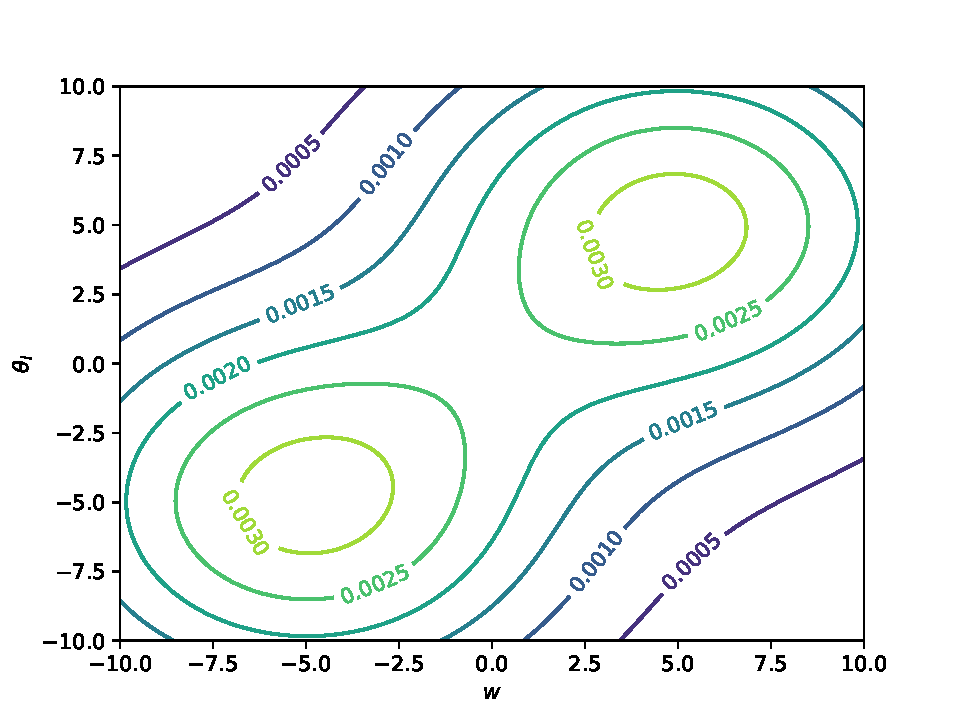
\includegraphics[width=.5\textwidth]{include/figures/plot2}
    \caption{Binormal plot for two strong up-/downdrafts with increased standard deviations}
    \label{fig:plot2}
    $w_1 = 5$, $w_2 = -5$, $\theta_{l1} = 5$, $\theta_{l2} = -5$,
    $\alpha = 0.5$, $\sigma_w = 5$, $\sigma_{\theta_{l1}} = 5$, $\sigma_{\theta_{l1}} = 5$.
\end{figure}
Seeing \cref{fig:plot2},
the issue with having some values in the middle is mitigated
but the general width of the normals was increased, too.
Since \gls{CLUBB} also has the simplification
that there is no correlation between $w$ and $\theta_l$,
and $w$ and $r_t$ -- obviously -- one cannot just increase it.
Therefore, the idea is to add this third normal distribution,
which actually has correlation between all three variables
and especially in the bivariate case, between $w$ and $\theta_l$.
\Cref{fig:plot2} would then change to \cref{fig:plot3}.
\begin{figure}[!htb]
    \centering
    \begin{tabular}{cc}
        \multicolumn{1}{c}{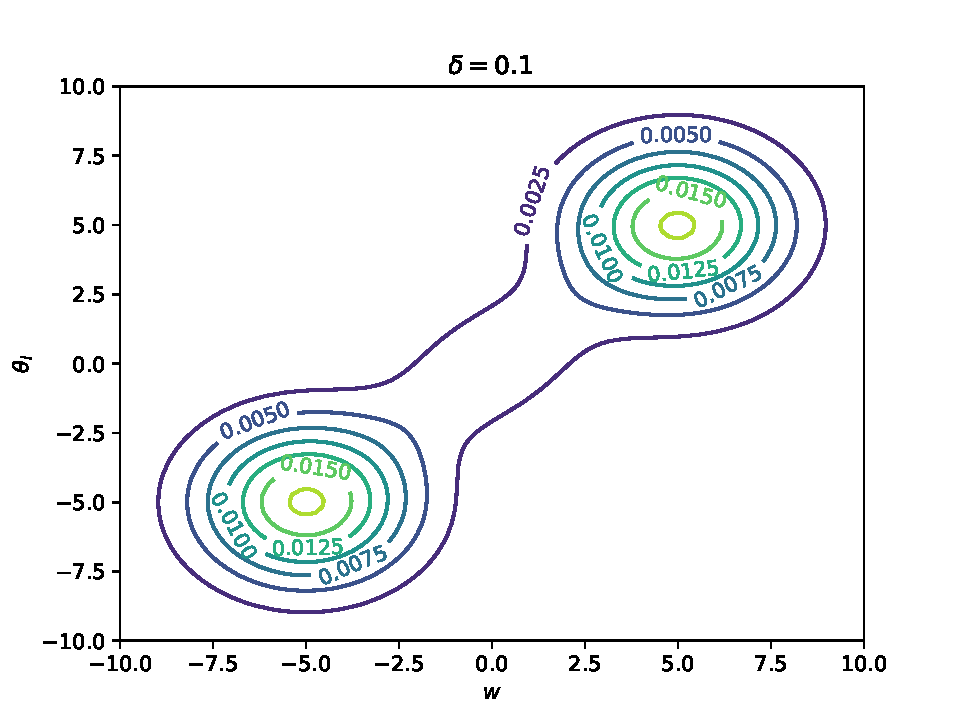
\includegraphics[width=0.47\textwidth]{include/figures/plot3_1}} &
        \multicolumn{1}{c}{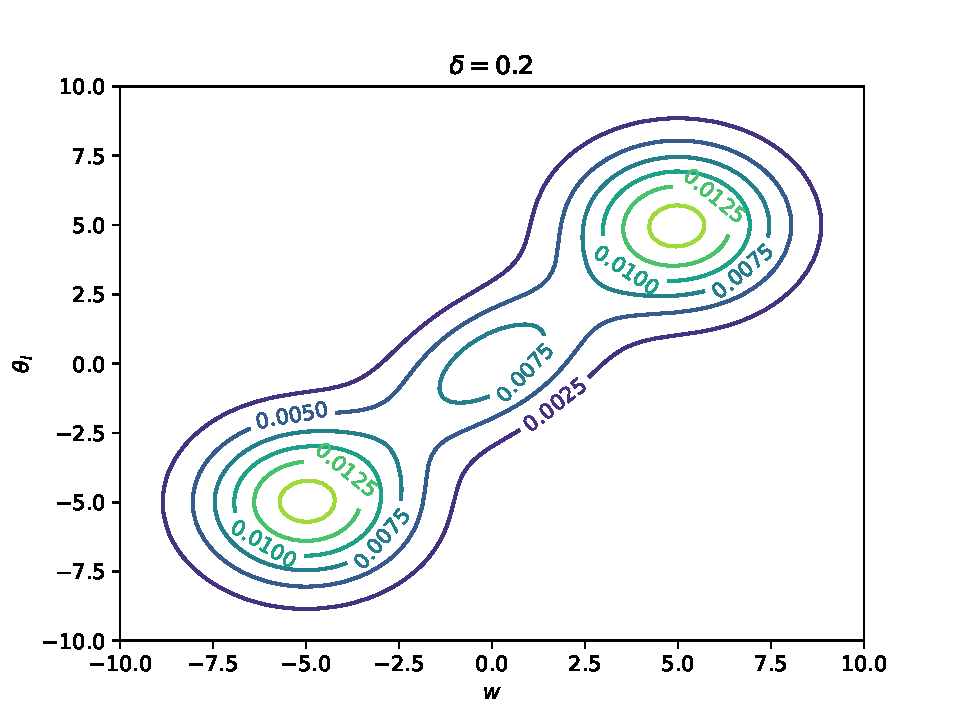
\includegraphics[width=0.47\textwidth]{include/figures/plot3_2}} \\
        \multicolumn{1}{c}{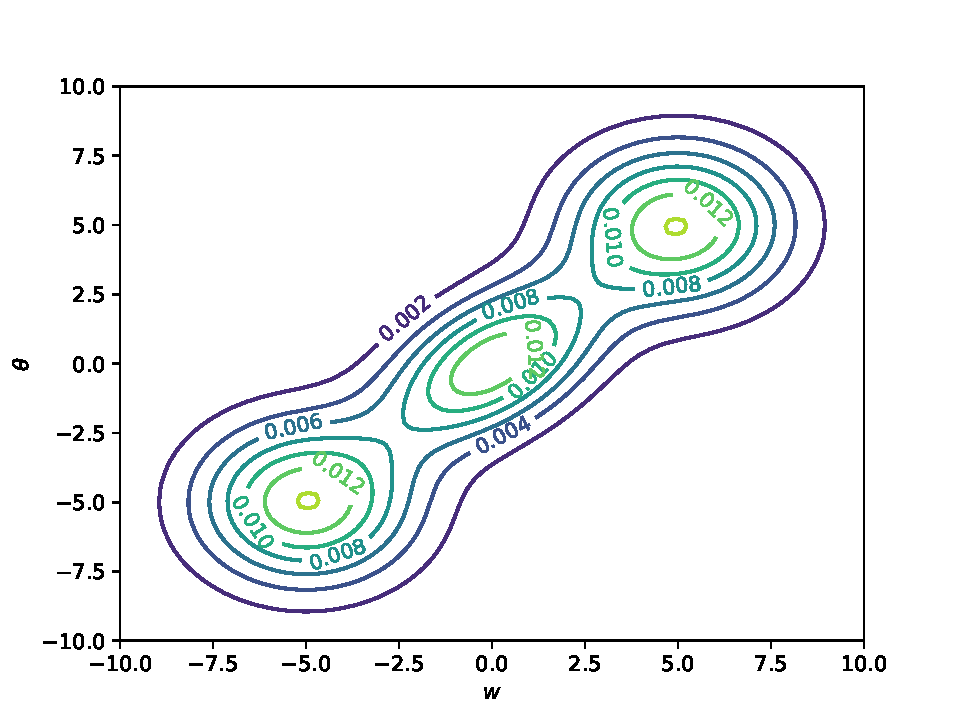
\includegraphics[width=0.47\textwidth]{include/figures/plot3_3}} &
        \multicolumn{1}{c}{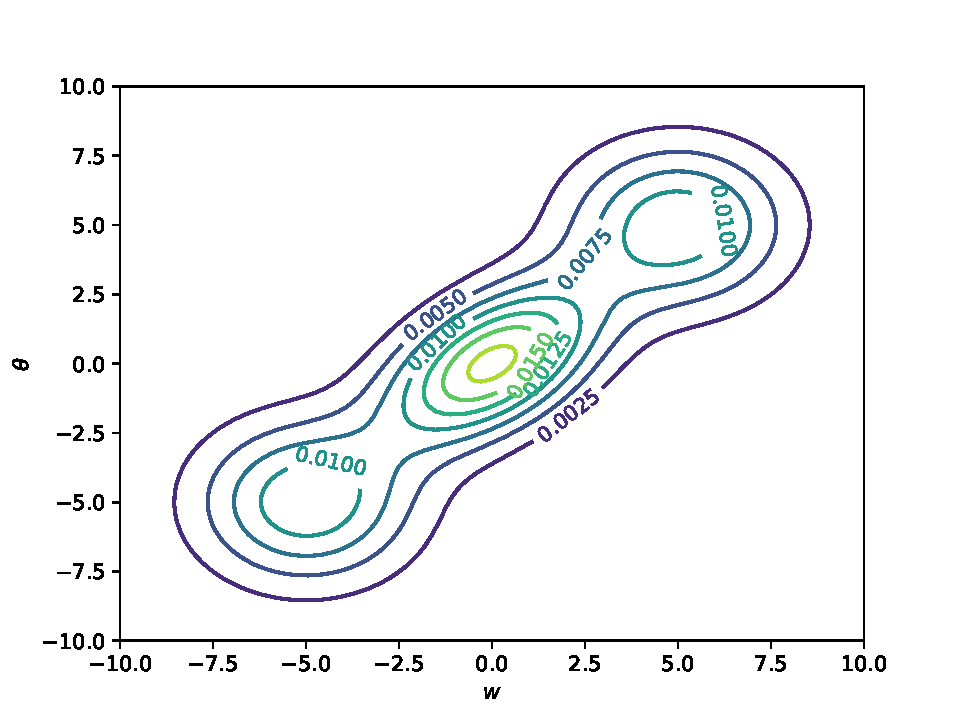
\includegraphics[width=0.47\textwidth]{include/figures/plot3_4}} \\
    \end{tabular}
    \caption{Trinormal plot for two strong up-/downdrafts with varying $\delta$}
    \label{fig:plot3}
    $w_1 = 5$, $w_2 = -5$, $\theta_{l1} = 5$, $\theta_{l2} = -5$,
    $\alpha = 0.5$, $\sigma_w = 2$, $\sigma_{\theta_{l1}} = 2$,  $\sigma_{\theta_{l2}} = 2$,
    $\sigma_{w3} = 2$, $\sigma_{3\theta_l} = 2$, $\rho_{w\theta_l} = 0.5$.
\end{figure}
Now, one can easily model something like the described shape,
as illustrated in \cref{fig:plot3}.
Also, some other (maybe weird) shapes are now possible,
just like the one in \cref{fig:plot4}.
\begin{figure}[!htb]
    \centering
    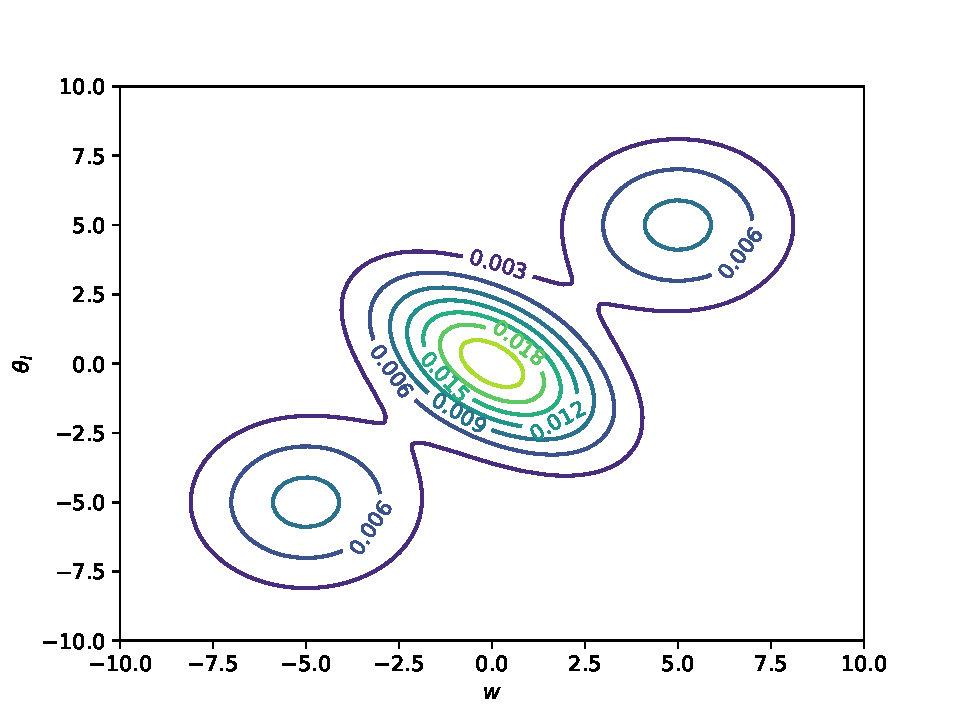
\includegraphics[width=.5\textwidth]{include/figures/plot4}
    \caption{Trinormal plot for two strong up-/downdrafts with a third peak in the middle}
    \label{fig:plot4}
    $w_1 = 5$, $w_2 = -5$, $\theta_{l1} = 5$, $\theta_{l2} = -5$,
    $\alpha = 0.5$, $\delta=0.5$, $\sigma_w = 2$, $\sigma_{\theta_{l1}} = 2$,
    $\sigma_{\theta_{l2}} = 2$, $\sigma_{w3} = 2$, $\sigma_{\theta_l 3} = 2$,
    $\rho_{w\theta_l} = 0.5$.
\end{figure}
